\documentclass{article}
\usepackage[utf8]{inputenc}
\usepackage{amsmath}
\usepackage{graphicx}
\usepackage{physics}
\begin{document}
\section{Problem 2 within project 1}
We are looking to write a program that defines a vector of x-values, and a function that evaluates the excact solution over these values, the results of which
will be stored in 2 columns, with a fixed amount of decimals, in scientific notation. This data will also be plotted separately.
\subsection*{excact solution}
we require a function that returns $u(x)$ for an input $x$, such that:
\begin{align}    
    \label{eq:excact_solution}
    u(x) =  1 - (1-e^{-10})x - e^{-10x}
\end{align}
A function "analytic\_sol" is declared of type double, and so is it's (only) parameter "x". the function body evaluates and returns x within 
\ref{eq:excact_solution}.


\begin{figure}
    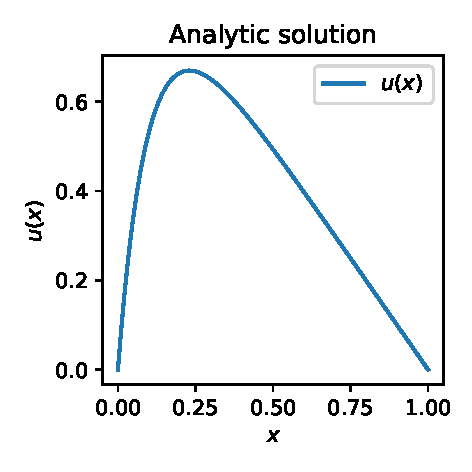
\includegraphics{problem_2_fig.pdf}
    \caption{Shows 100 linearly spaced points between 0 and 1, evaluated on the excact solution $u(x)=1 - (1 - e^{-10})x - e^{-10x}$.}
\end{figure}


\end{document}